\def\theTopic{Testing Slope = 0 }
\def\dayNum{18 }

\begin{center}

{\bf {\large Is Correlation Zero?  Is Slope Zero?}}
\end{center}

Recall the plots we started with last time of ``most attractive age'':
\vspace{-.5cm}

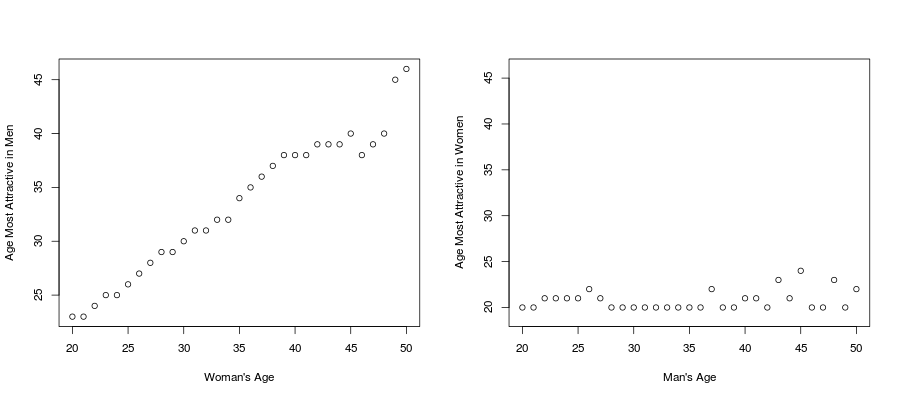
\includegraphics[width=\linewidth]{../../plots/attractiveAges.png}

Least squares regression lines:
$$ \mbox{Women: } \hat{y} = 9.02 + 0.70x \mbox{ \hspace{2in}}
   \mbox{Men: } \hat{y} = 19.57 + 0.0343x \mbox{ \vspace{-.7cm}} $$ 
\begin{enumerate}
  \item What would you guess  women aged 36.5 would say is the
    most attractive age of men? 
\begin{students}
 \vspace{1.5cm}      
\end{students}

\begin{key}
  {\it     Plug 36.5 in as the x value and compute $\hat{y} = 34.47$.}
\end{key}

  \item What would you guess  men aged 49.5 would say is the
    most attractive age of women? 
\begin{students}
 \vspace{1.5cm}      
\end{students}

\begin{key}
  {\it     Plug 49.5 in as the x value and compute $\hat{y} = 21.27$.}
\end{key}

\item Discuss this alternative with your group.  Perhaps the age of
  the men really doesn't matter, and we'd be better off estimating
  their preference by using the mean ``most attractive age for women''
  which is $\overline{y} = 20.78$ for all men, just ignoring the men's age.
   Does that seem like a reasonable way to describe the second plot:
   ``men of all ages find 20.8 years to be the most attractive in women''?
  Write down your group's conclusion.
  \begin{students}
 \vspace{2cm}      
\end{students}

\begin{key}
  {\it    I hope they can see some validity in both regression line
    and flat line.}
\end{key}

  BTW: If any of you women over age 23 find this depressing, Rudder
  does say in his book that when men go to search for women on the
  dating site, they do adjust for their own age and ask to see
  profiles of older women if they are older themselves.  % Also, our $y$
  % values are averaged over a bunch of men of the same age. If we used
  % data from individuals, the relationship would be even weaker.


\item Go to the website
  \url{http://shiny.math.montana.edu/jimrc/IntroStatShinyApps/},
  select \fbox{Two Quant.} and ``Enter Data''. The OKcupid data is
  preloaded as either {\tt WomenRateMen} or {\tt MenRateWomen}. Use
  the men's rating of women for now.

Consider this line:
  {\it  $\widehat{mostAttrWomen} = 20.77 + 0 \times $ mansAge   }


    \begin{enumerate} 
    \item Where have you seen the intercept estimate before?

      \item If you plug in any age for men, say 18 or 54, what result
        will you get from this line?
\begin{students}
 \vspace{1.cm}      
\end{students}

\begin{key}
  {\it   20.77    }
\end{key}
      \item What does that say about the relationship between $x$ and
        $y$?
\begin{students}
 \vspace{1.cm}      
\end{students}

\begin{key}
  {\it  $y$ does not depend on $x$  }
\end{key}

      \item What will be the true slope for $y$ based on $x$ if there
        is no relationship?  Use    correct notation.
\begin{students}
 \vspace{1cm}      
\end{students}

\begin{key}
  {\it  $\beta_1=0$   }
\end{key}
      \end{enumerate}
      

\item  If we  want to test the null hypothesis ``no linear
  relationship between men's age and the age of women they find most
  attractive'', what is the null value of the true slope?  Use $\beta_1$ as the
  true slope and fill in the hypotheses.  Use a ``right-tailed'' alternative.\\
  $H_o:$
\begin{students}
 \vspace{1cm}      
\end{students}
\begin{key}
  {\it  $\beta_1 = 0$   }
\end{key}

  $H_a$
\begin{students}
 \vspace{1cm}      
\end{students}
\begin{key}
  {\it  $\beta_1 > 0$   }
\end{key}

\item When you select ``Test'' for these data, a ``Shuffled Data''
  plot appears in the middle of the page. For each $x$ value, there is
  a line from the original (blue) y value to the new shuffled $y$
  value (green).   Does this shuffle follow $H_0$ or $H_a$?  Explain.
\begin{students}
 \vspace{1cm}      
\end{students}

\begin{key}
  {\it  Y's are shuffled. If $H_0$
  is true, then there is no linear association between $x$ and $y$, so
the shuffled data could have occurred just by chance.}
\end{key}

% \item Change Data to Plot. The red line comes from where? 
% \begin{students}
%  \vspace{1cm}      
% \end{students}

% \begin{key}
%   {\it  It's the least squares line from the left-hand plot of the
%     original data.   }
% \end{key}
\item %Run several  shuffles, then several 1000.  
Is the least squares line in the lower plot  flatter or steeper than
the one  in the upper plot?  Is $\hat{\beta}_1$ closer or further
from zero? 
\begin{students}
 \vspace{1cm}      
\end{students}

\begin{key}
  {\it AWV.  generally flatter}
\end{key}

\item  Take at least 1000 shuffles and compute the p-value.  Explain
  which shuffles you are counting. 
\begin{students}
 \vspace{2cm}      
\end{students}

\begin{key}
  {\it In 10000 shuffles, I had 549 with slope greater than 0.0343, so
  my p--value is 0.055}
\end{key}

\item State your decision and conclusion using $\alpha = 0.05$.
\begin{students}
 \vspace{2cm}      
\end{students}

\begin{key}
  {\it At the $\alpha = 0.05$ significance level we do not reject
    $H_0$, We have only moderate evidence that the true slope between
    men's age and the age of woman they find most attractive is
    greater than zero.  In other words: There is a weak positive
    association between the two variables which is not significant at
    the 0.05 level.}
\end{key}

\item Switch from slope to correlation. What is the sample
  correlation, and what is the p-value for a test of $H_0:\ \rho=0$
  versus $H_a:\ \rho > 0$?.
\begin{students}
 \vspace{1cm}      
\end{students}

\begin{key}
{\it $r = 0.287$ and the p-value is the same.}
\end{key}

\item Now test to see if slope is zero when we compare women's age
  (now this is $x$) to the age of men they find most attractive (our
  new $y$). Again use a ``right-tailed'' alternative.  
  \begin{enumerate}
  \item State the hypotheses.\\
  $H_o:$
\begin{students}
 \vspace{1cm}      
\end{students}
\begin{key}
  {\it  $\beta_1 = 0$   }
\end{key}

  $H_a$
\begin{students}
 \vspace{1cm}      
\end{students}
\begin{key}
  {\it  $\beta_1 > 0$   We don't expect a negative relationship.}
\end{key}

  \item Go back to ``Enter Data'' and load the women's data.  What is
    the equation of the least squares line?
\begin{students}
 \vspace{1cm}      
\end{students}

\begin{key}
  {\it $\widehat{mostAttrMen}$ = 9.02 + 0.6972 x womansAge}
\end{key}


  \item Create 1 random shuffle of the data.  Explain (yes, again --
    it's important)  what is being shuffled. 
\begin{students}
 \vspace{1.8cm}      
\end{students}

\begin{key}
  {\it Use the same woman's ages from 20 to 50. Shuffle the ages of the
    men each woman finds most attractive ($y$)}
\end{key}

  \item Compute the p--value and interpret it.
\begin{students}
 \vspace{1cm}      
\end{students}

\begin{key}
  {\it I get 0. In 10000 shuffles, none was as extreme as the slope we
    observed. The p-value is the probability of seeing a slope this
    far above 0 if, in fact, woman's age ($x$) and most attractive
    man's age ($y$) are really unrelated (true $\beta_1=0$).}
\end{key}


\item State your decision and conclusion using $\alpha = 0.05$.
\begin{students}
 \vspace{2cm}      
\end{students}

\begin{key}
  {\it At the $\alpha = 0.05$ significance level we  reject
    $H_0$, We have super strong evidence that the true slope between
    women's age and the age of man they find most attractive is
    greater than zero.  In other words: There is a very strong positive
    association between the two variables which is significant at
    the 0.05 level.}
\end{key}

 
\item Switch from slope to correlation. What is the sample
  correlation, and what is the p-value for a test of $H_0:\ \rho=0$
  versus $H_a:\ \rho > 0$?.
\begin{students}
 \vspace{1cm}      
\end{students}

\begin{key}
{\it $r = 0.982$ and the p-value is the same.}
\end{key}
  \end{enumerate}

  
\item Are the men and women shown in these plots a random sample from
  a larger population?  Are they representative of some larger population?
\begin{students}
 \vspace{2cm}      
\end{students}

\begin{key}
  {\it No.  The data are averaged across each age, and we can't say
    that the people using this dating site represent a larger
    population of singles.}
\end{key}

\item Was some  treatment  randomly assigned?
\begin{students}
 \vspace{1.5cm}      
\end{students}

\begin{key}
  {\it No.  The ``explanatory'' ages ($x$ values) were observed for
    each person, not assigned.} 
\end{key}

\item What is the scope of inference?
\begin{students}
 \vspace{1.5cm}      
\end{students}

\begin{key}
  {\it We can only say there is ( for women,  is not for men)
    evidence of association in these samples of singles.} 
\end{key}

\item Write a report on the two hypothesis tests we just did. \vfill
\end{enumerate}
 

\begin{center}
  {\bf Take Home Messages:}\vspace{-.4cm}
\end{center}
\begin{itemize}
  \item A slope of zero is very ``special'' in that is says we would
    predict the same value for the response, $\hat{y}$ for all values
    of $x$.  That means that there is no linear relationship between
    the two variables.
  \item The OKCupid data gives us one example where slope is close to
    zero and another where slope is far from zero.  Our conclusions
    should be quite different.
  \item The mechanics of computing p--value have not changed.  We
    assumed $H_0$ was true, and created shuffled data consistent with
    $H_0$.  For each dataset, we computed a slope, and plotted a
    histogram for slopes under $H_0$. P--value counted the number of
    times a slope was as or more extreme as the one we observed
    divided by the number of shuffles.  The only difference is that we
    had the computer find slopes instead of proportions or means.  You
    can easily click the correlation button to get a test of $H_0:\ \
    \rho = 0$. P--values will agree with the test for slope = 0.
 \item 
  Use the remaining space for any questions or your own summary of the
  lesson. \vspace*{\fill}

\end{itemize}

